% Independent native probes for the real half-plane tick pipeline.
\makeatletter
\newcount\ticknumber
\newcommand{\probepolartick}{%
  \global\advance\ticknumber by1
  \pgfextractx{\dimen0}{\pgfpointanchor{\tikzlastnode}{center}}%
  \pgfextracty{\dimen2}{\pgfpointanchor{\tikzlastnode}{center}}%
  \typeout{POLAR-CENTER \the\ticknumber: \the\dimen0,\the\dimen2}%
  \typeout{POLAR-ORIGIN \the\ticknumber: \meaning\pgf@dv@tick@origin}%
  \typeout{POLAR-DIR \the\ticknumber: \meaning\pgf@dv@tick@dir}%
  \typeout{POLAR-ANGLE \the\ticknumber: \lastpolarangle}}
\AtBeginDocument{%
  \pgfdvmathenter{\a}{1.8}\pgfdvmathenter{\b}{0.03141592653589793}%
  \pgfdvmathdiv{\c}{\a}{\b}%
  \pgfdvmathexitbyscientificformat{\c}{\c}\typeout{POLAR-RAD-SCALE: \c}%
  \let\nativesincos\pgfmathsincos
  \def\pgfmathsincos#1{\xdef\lastpolarangle{#1}\nativesincos{#1}}%
  \let\nativearcaxes\pgfpatharcaxes
  \def\pgfpatharcaxes#1#2#3#4{%
    \nativearcaxes{#1}{#2}{#3}{#4}%
    \pgfgetpath\nativearcpath
    \typeout{POLAR-ARC #1:#2: \meaning\nativearcpath}}%
  \tikzdatavisualizationset{every ticks/.append style={node style={append after command={\pgfextra{\probepolartick}}}}}}
\makeatother
\documentclass[border=2pt]{standalone}
\usepackage{tikz}
\usetikzlibrary{datavisualization.formats.functions,datavisualization.polar}
\begin{document}
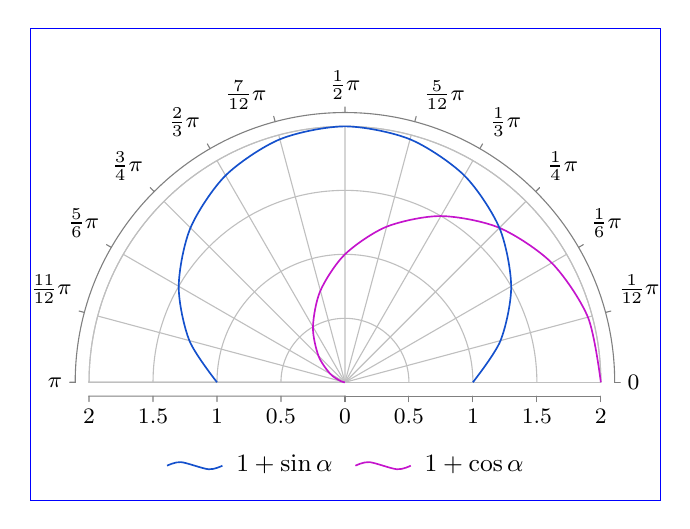
\begin{tikzpicture}
  \draw[blue,line width=.2pt] (-4,-1.5) rectangle (4,4.5);
  \datavisualization [scientific polar axes={0 to pi,clean},all axes=grid,
    style sheet=vary hue,legend=below]
    [visualize as smooth line=sin,sin={label in legend={text=$1+\sin\alpha$}}]
    data [format=function] {
      var angle : interval [0:pi] samples 13;
      func radius = sin(\value{angle}r) + 1;
    }
    [visualize as smooth line=cos,cos={label in legend={text=$1+\cos\alpha$}}]
    data [format=function] {
      var angle : interval [0:pi] samples 13;
      func radius = cos(\value{angle}r) + 1;
    };
\end{tikzpicture}
\end{document}

